\chapter{Subsystems}
\label{chap:subsystems}
.....



\section{Rover}
\label{sec:rover}
...
\section{Structure and Mechanics}
\label{sec:mechanics}
...
\section{Communications and Command and Data-Handling}
\label{sec:comm}
...
\section{Payload}
\label{sec:payload}
...
\section{Thermal Control}
\label{sec:thermalcontrol}
...
\section{Electrical Power System}
\label{sec:EPS}
The EPS (Electrical Power System) is the subsystem responsible for the electrical power supply of INSPIRE. It consists of four funadmental parts, which are the energy source, the PCDU unit (Power Control and Distribution)and the Energy Storage as well as the rover subsystems as the consumers.

\subsection{EPS Budget and Overview}

\begin{figure}[htb]
{\centering
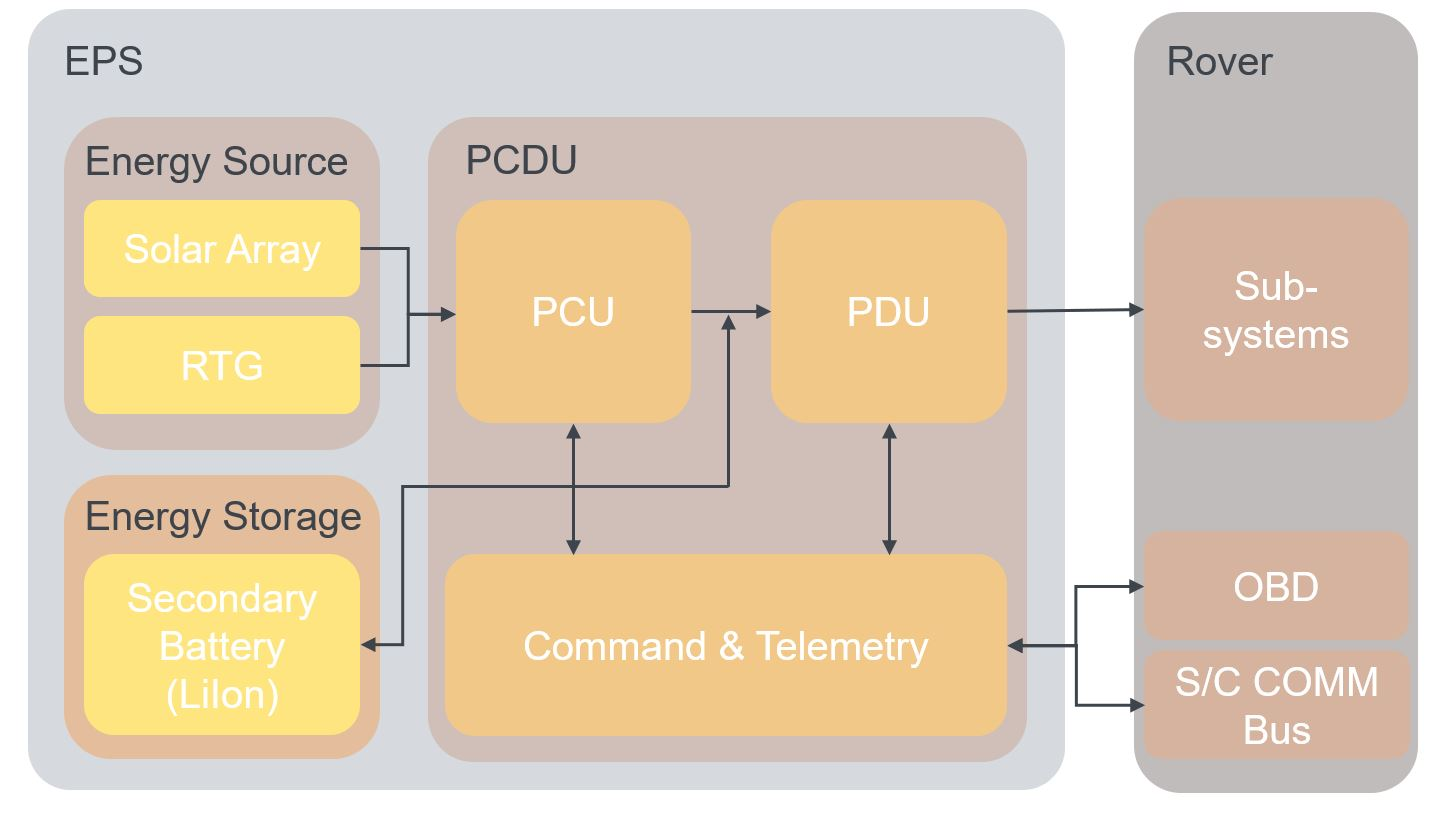
\includegraphics[width=0.7\textwidth]{Media/epsflowchart}
\caption{Functional Flow Chart Diagram for the EPS Subsystem.}
\label{fig:epsflowchart}
}
\end{figure}

\subsection{EPS Power Control and Distribution}

\subsection{Energy Source}
For the energy generation of INSPIRE many possible sources were taken into consideration a trade-off. The outcome of this trade-off is shown in \autoref{fig:epssourcetradeoff} for the most promising energy sources. As a conclusion of this trad-off the decision was made to utilize a Radioisotope Thermoelectric Generator (RTG) as the main energy source for INSPIRE. \\

As the research couldn't find an RTG with a mass suitable for INSPIRE, the solution was to scale down a bigger RTG as an approximation. As a baseline of the scaling the eMMRTG (Enhanced Multi Mission Radioisotope Thermoelectric Generator) was utilized, which is currently under development at NASA and is especially designed for deep space missions like Europa. For the scaling a goal RTG mass of 3 kg was defined and the eMMRTG was scaled down using the given data.
In \autoref{tab:esmmrtg} the scaling results for the eSMMRTG (Enhanced and Scaled Multi Mission Radioisotope Thermoelectric Generator) are listed. The eSMMRTG has a mass of 3 kg and a BOL specific power of 3.6 w/kg as well as a electrical power of 12.08 Watts during the mission duration and a thermal power of roughly 142.1 Watts.



\begin{figure}[htb]
{\centering
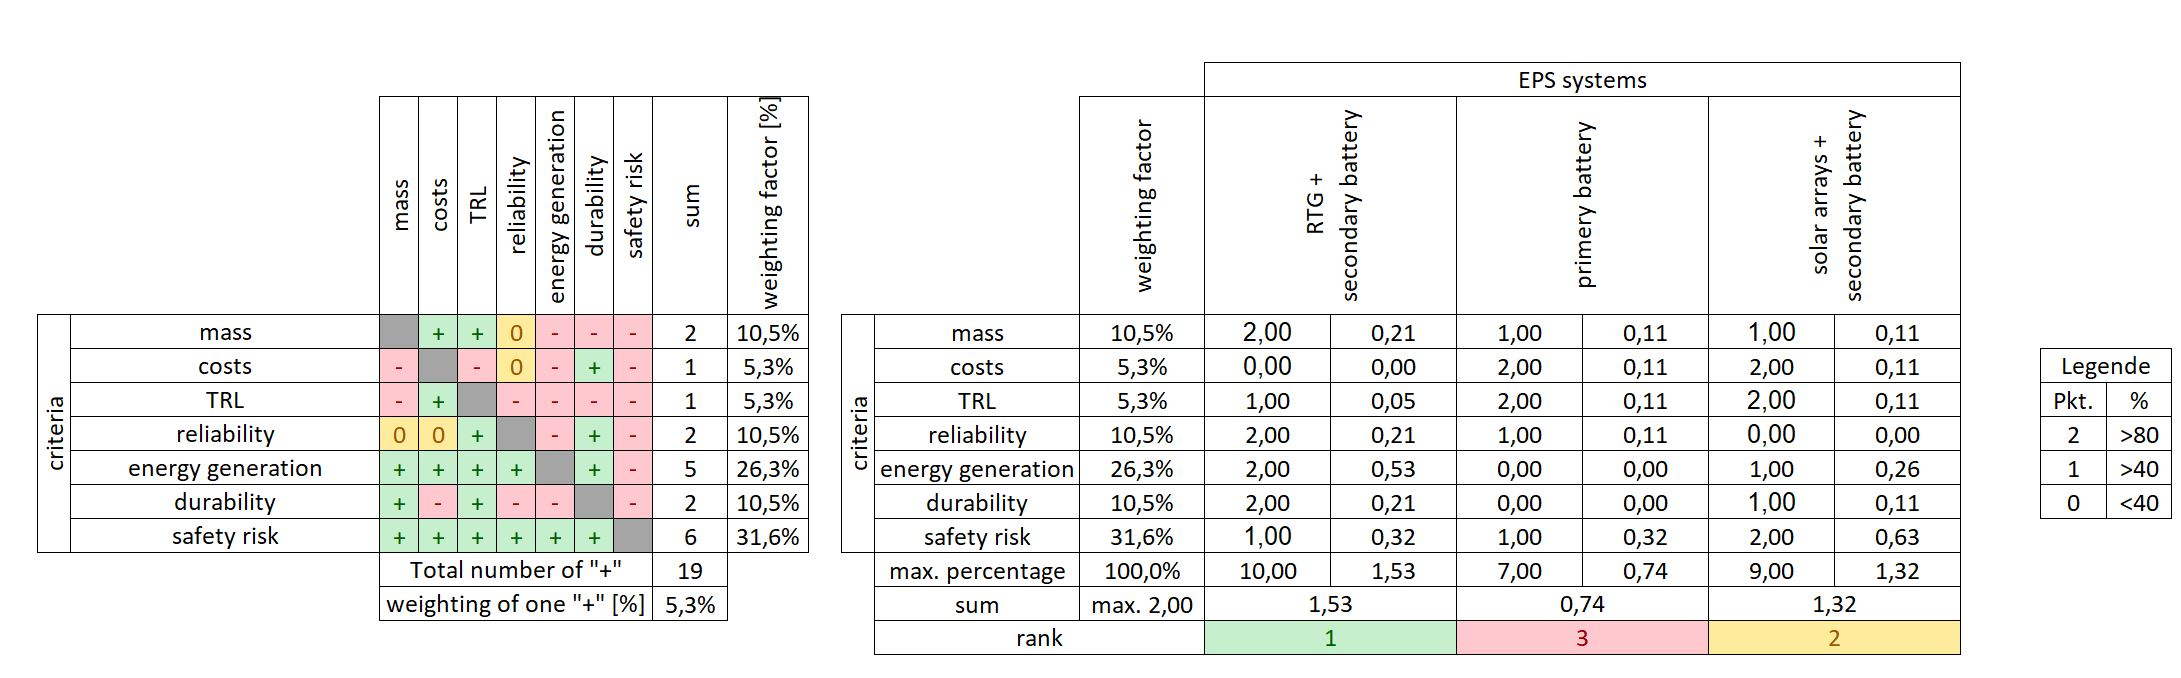
\includegraphics[width=0.7\textwidth]{Media/epssourcetradeoff}
\caption{Trade-Off Conclusion for the EPS Energy Source.}
\label{fig:epssourcetradeoff}
}
\end{figure}

\begin{table}[H]
\centering
\begin{tabular}{|c|c|}
\hline
\multicolumn{2}{|c|}{Scaled eSMMRTG Parameter}                \\ \hline
Isotrop                                            & Pu-238   \\ \hline
Isotrop Half-Life {[}a{]}                          & 87.7     \\ \hline
Flight time and Storage incl. Margins  {[}a{]}     & 7        \\ \hline
Begin of Life Power P\_el,BOL {[}W\_el{]}          & 14       \\ \hline
Power Loss Degradation until BOM {[}W{]}           & 0.56     \\ \hline
Begin of Mission Power P\_el,BOM {[}W\_el{]}       & 13.44    \\ \hline
Europa Day Duration {[}h{]}                        & 85       \\ \hline
Mission Duration {[}d{]}                           & 106.25   \\ \hline
End of Mission Power P\_el,EOM {[}W\_el{]}         & 13.42    \\ \hline
Final Power for Study P\_el {[}W\_el{]}            & 12.08    \\ \hline
Design Point BOL Heat Generation Q\_HS {[}W\_Th{]} & 142.1053 \\ \hline
BOL Specific Power {[}w\_el /kg{]}                 & 4.0      \\ \hline
System Mass {[}kg{]}                               & 3.5      \\ \hline
\end{tabular}
\caption{Parameters for the scaled eSMMRTG based on the eMMRTG}
\label{tab:esmmrtg}
\end{table}


\subsection{Energy Storage} 



\clearpage

\section{Radiation}
\label{sec:Radiation}

Compared to the radiation environment near Earth the radiation environment near Jupiter is multiple times stronger. It has the highest radiation levels of any planet in our solar systems \cite{Platzhalter}. In order to survive these harsh environmental conditions, special emphasis must be placed on the radiation protection. In \autoref{fig:trappedprotonelectronfluxes}, the average trapped proton and electron fluxes on Europa's orbit around Jupiter are shown in comparison to the outer Van Allen radiation belt around Earth. However, in contrast to the Van Allen radiation belt, the duration within the radiation environment on Europa cannot be minimised and the rover has to be designed to withstand the entire mission duration of 30 days.

\begin{figure}[htb]
     \centering
     \begin{subfigure}[b]{0.475\textwidth}
         \centering
         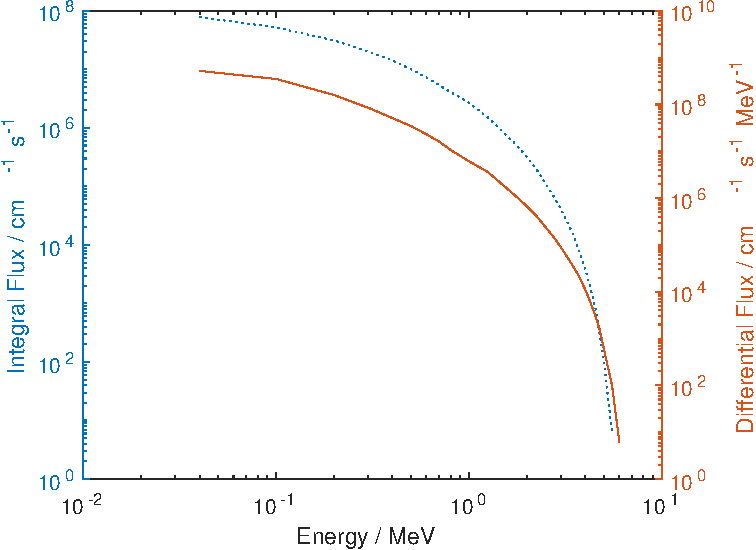
\includegraphics[width=\textwidth]{Media/E_Electron_Flux}
         \caption{Average spectra of trapped electrons around Earth.}
         \label{fig:trappedelectronsEarth}
     \end{subfigure}
     \hfill
     \begin{subfigure}[b]{0.475\textwidth}
         \centering
         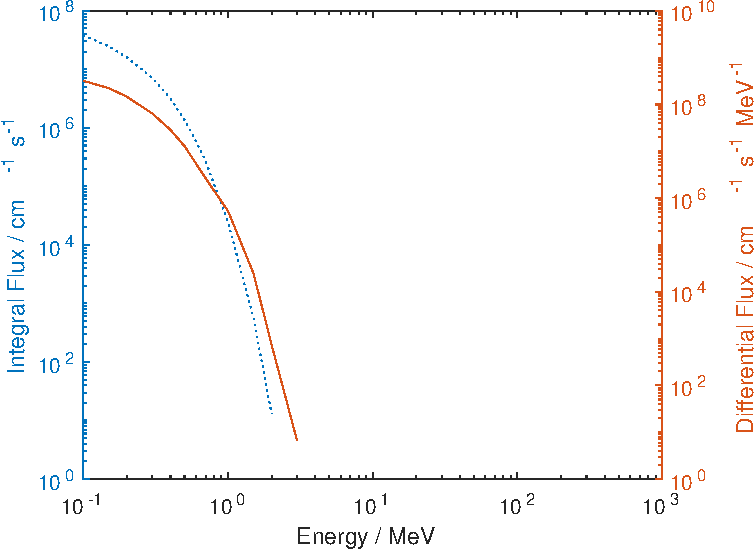
\includegraphics[width=\textwidth]{Media/E_Proton_Flux}
         \caption{Average spectra of trapped protons around Earth}
         \label{fig:trappedprotonsEarth}
     \end{subfigure}
     \hfill
     \begin{subfigure}[b]{0.475\textwidth}
         \centering
         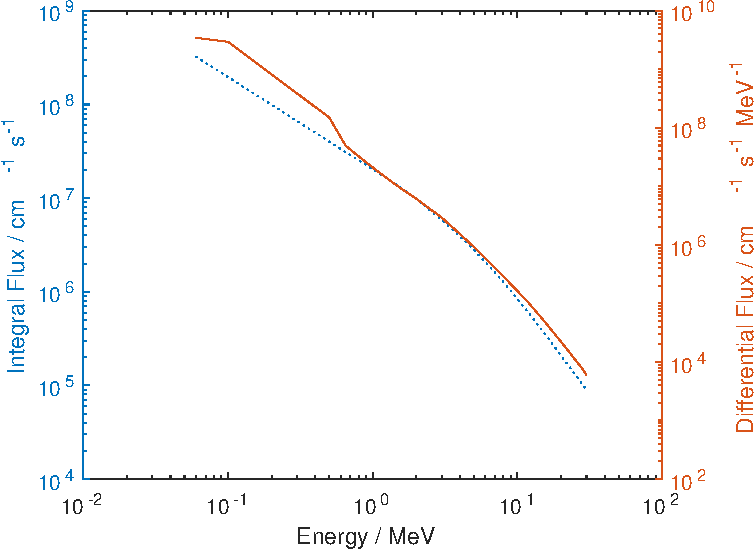
\includegraphics[width=\textwidth]{Media/J_Electron_Flux}
         \caption{Average spectra of trapped electrons around Jupiter}
         \label{fig:trappedelectronsJupiter}
     \end{subfigure}
     \hfill
     \begin{subfigure}[b]{0.475\textwidth}
         \centering
         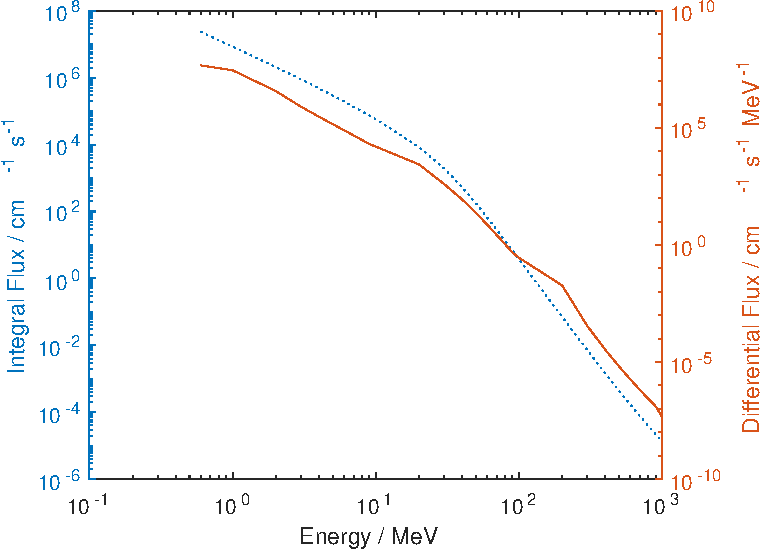
\includegraphics[width=\textwidth]{Media/J_Proton_Flux}
         \caption{Average spectra of trapped protons around Jupiter}
         \label{fig:trappedprotonsJupiter}
     \end{subfigure}
        \caption{Average trapped proton and electron fluxes on an orbit around earth at 25,000 km, through the outer Van Allen radiation belt, and on Europa's orbit around Jupiter.}
        \label{fig:trappedprotonelectronfluxes}
\end{figure}

In oder to design and evaluate different radiation protection approaches, different calculations have to be performed. For this purpose the ESA SPace ENVironment Information System (SPENVIS) is used \cite{Platzhalter}. All calculations and figures in \autoref{sec:Radiation} are performed with SPENVIS unless otherwise stated.

\section{Locomotion}
\label{sec:locomotion}

\section{Control and Autonomy}
\label{sec:ControlandAutonomy}

\cleardoublepage